\section{Transfer between halos}
\label{sec:transfer}

Looking at particle-level metrics can be informative, but the majority of
analysis performed on cosmological simulations occurs on bound structures for
good reason; they are what can be accurately observed and easily identified.
The below analysis considers transfer of baryonic material between halos and
their associated lagrangian regions in the initial conditions of the
simulation.

\subsection{Defining halos}

Halos in the following discussion are defined by using the \velociraptor{} structure
finder \citep{Elahi2019}. This structure finder uses a 6D friends-of-friends (FoF) algorithm
with an adaptive linking length for each halo to disentangle mergers. A standard
linking length of $\ell = 0.2$ is used for the initial 3D FoF search for field halos.
The parameter files that were used to find the halos can be found on our \github{}
page here\footnote{\url{https://github.com/jborrow/simba-velociraptor-tools} using
revision {\tt 6444583}} and used the revision {\tt baa2c2c} of
\velociraptor{}. As the analysis presented here uses halo-level metrics, no galaxy
finder was used, and \velociraptor{} was not ran in galaxy-finding mode.

\subsection{Defining lagrangian regions}


Many methods exist for defining lagrangian regions, but these are mostly used for
zoom-in simulations and some, for example using a cube of particles around a given
halo, could be seen as being non-lagrangian and over-conservative. In the below
discussion the lagrangian regions are defined in the initial conditions in the
following way:
\begin{enumerate}
	\item Find all halos at $z=0$.

    \item For each halo, ID match the particles contained within it with those
		  in the initial conditions. This defines the initial lagrangian region
		  based on the dark matter.

	\item In some cases, discussed below, fill in the holes in this lagrangian
	      region by using a nearest-neighbour search.

	\item For every gas particle in the initial conditions, find the nearest dark
	      matter neighbour. This gas particle is assigned to the same lagrangian
	      region as that dark matter particle.
\end{enumerate}
This allows the definition of the lagrangian region to also extend to the gas
that should be gravitationally bound by that halo at $z=0$. For results quoted
at higher redshifts, the above approach is repeated, except the halos are
found at the quoted redshift and the particle data from that snapshot is used.
There is no attempt made to lagrangian-region match, i.e. the lagrangian regions
that are defined at $z=2$ have no relation to the ones at $z=0$ other than that
they are from the same simulation.

\subsection{Calculating transfer between lagrangian regions}

Now that the lagrangian regions have been defined, it is possible to consider on
a particle-by-particle basis where particles started and where they ended up.
The algorithm is as follows:
\begin{enumerate}
	\item ID match all particles between the initial and final conditions, including
	      star particles (these are matched to their gas progenitor). Black holes
	      are ignored in this analysis.

	\item Every particle in the $z=0$ final conditions has several possible final
	      states and origins, based on its halo ID $i$:
	      \begin{itemize}
	            \item Particle resides in a halo $i$
	            \begin{itemize}
	           		\item Particle originated in the same lagrangian region $j = i$
	           		\item Particle originated outside any lagrangian region $j = -1$
	           		\item Particle originated in some other lagrangian region $j \neq i$
	            \end{itemize}
	            \item Particle resides outside a halo ($i = -1$)
	            \begin{itemize}
	            	\item Particle has never been in any lagrangian region or halo
	            	\item Particle originated in a lagrangian region $j$ and was moved out
	            \end{itemize}
	      \end{itemize}
	      
	\item For every halo and lagrangian region the mass originating from each
	      of the above compopnents is computed and stored.
\end{enumerate}

The source code that performs all of the above analysis is made available by
the authors on \github{}\footnote{\url{https://github.com/jborrow/lagrangian-
transfer}} as a python package.

\subsection{Transfer in a non-radiative Model}

\begin{figure}
	\centering
	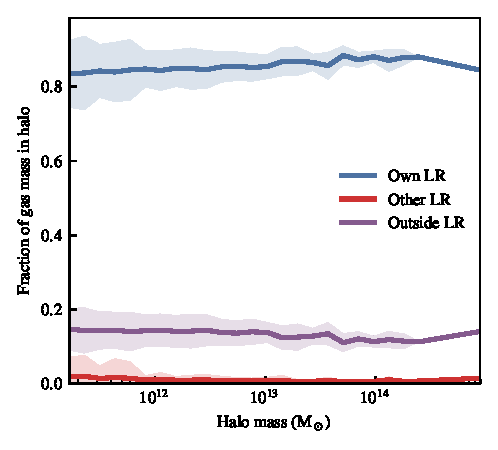
\includegraphics[width=\columnwidth]{figures/s50gadget/component_fraction_vs_halo_mass_gas.pdf}
	\vspace{-0.7cm}
	\caption{
	The fraction of baryonic mass originating from each lagrangian component is
	shown as a function of redshift $z=0$ halo mass, later referred to as the
	Baryon Transfer Mass Function (BTMF). This is only provided for comparison to
	the full model result in Fig. \ref{fig:maintransferresult}.
	}
	\label{fig:nonradiativetransfer}
\end{figure}

To begin with, let us consider a null model. In this case, we run the simulation
in non-radiative mode; i.e. without cooling, star formation, or feedback. This
simulation only includes hydrodynamics, comsology, and gravity. In Fig.
\ref{fig:nonradiativetransfer} we present the fraction of baryonic mass for
each halo contributed from each lagrangian component, as a function of halo
mass. There is no dependence on halo mass (as the simulation is effectively
scale-free above some resolution limit), and apart from some small level of 
transfer from outside any lagrangian region, the baryonic mass in each halo
consists of that which originated in its own lagrangian region.

\subsection{Transfer \emph{into} Halos}

\begin{figure*}
	\centering
	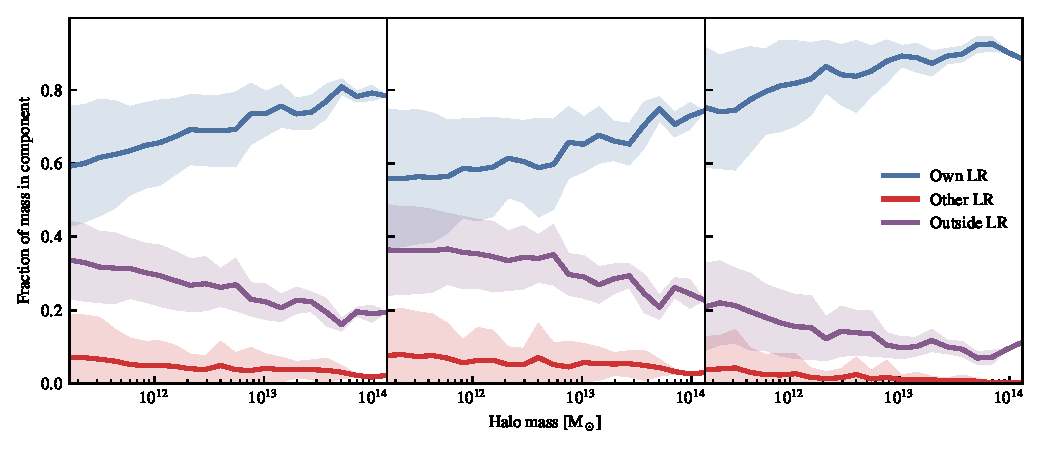
\includegraphics{figures/s50j7k/component_fraction_mixed.pdf}
	\vspace{-0.7cm}
	\caption{
		The fraction of baryonic mass originating from each lagrangian component is
		shown as a function of redshift $z=0$ halo mass, later referred to as the
		Baryon Transfer Mass Function (BTMF). Different panels show different
		particle selections with all baryonic
		mass (left), gas mass (center), and stellar mass (right). Shaded
		regions show the $1\sigma$ scatter in a given bin, with one standard
		deviation of variation being shown. There is no attempt made to include
		halo assembly bias or the finite halo sampling in a $50\hmpc{}$ box in
		these regions.
	}
	\label{fig:maintransferresult}
\end{figure*}

The results of the full model, transfer as a function of halo mass, are shown in Fig.
\ref{fig:maintransferresult}. The general trend is that for an increasing halo mass,
a lagrangian region is able to hold on to more of the original baryonic mass, with
this flattening off around $M_H = 10^{12} \msolar$. For a given halo, sigificantly
more of the gaseous mass originates outside the original lagranigan region as compared
to the stellar mass ($\sim 60 \%$ versus $\sim 90 \%$). The transfer between halos is
at around the $\sim 5-10\%$ baryonic mass level, with this transfer predominantly
originating from the gaseous component, as compared to the stellar component. This combines
nicely with the distnace metrics shown in \S \ref{sec:feedbackmetrics}, which
showed that the dark matter and stars have very similar dynamics and hence should be
similarly well bound. The physical reason for this is clear; many gas particles are ejected
by feedback events from halos, and are re-captured by other halos. These particles must then
be very hot (either through direct or shock heating) and so do not have the time to cool to
form stars at $z=0$.

The transfer between these regions is slightly lower, but is still at the $5-10\%$ level
even for the \nojet{} run. As shown by the non-radiative run in Fig. \ref{fig:nonradiativetransfer}, this is not simply a consequence of the definition of lagrangian region, or the dynamics (which are provably similar in terms of separation between dark matter and gas in a statistical sense, see Fig. \ref{fig:feedbackdistance}. This transfer is caused by the effects of the sub-grid (galaxy formation model).

In all of the relations there is a high level of scatter. The scatter in these
relations, as with other metrics in astronomy, likely contains more information 
than the relations themselves. A given mass bin contains halos that entertain a range
of 10x in transfer, which is likely dependent on environment. The specific physical
effects that lead to the scatter in these relations will be discussed in a follow-up
paper.

The overall fraction of baryonic mass that is retained by a given lagrangian
region does begin to turn over around $10^{13} \msolar{}$, however it is unclear
whether this is due to a lack of higher mass halos in the $50 \hmpc{}$ box. It
is also important to note that the shaded regions in Figure
\ref{fig:maintransferresult} represent the $1\sigma$ scatter in a given bin
and explicitly do \emph{not} include any errors that would occur from a finite
sampling of halos or halo assembly bias.

\begin{figure}
	\centering
	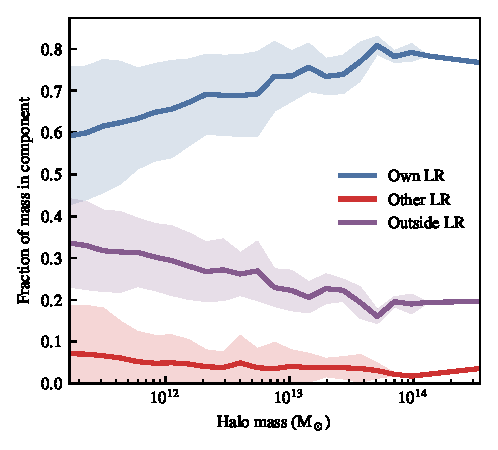
\includegraphics[width=\columnwidth]{figures/s50j7k_z2/component_fraction_vs_halo_mass_both.pdf}
	\vspace{-0.7cm}
	\caption{The BTMF for all baryons at redshift $z=2$, shown for
	the full \simba{} model. Note the very low proportion of mass transfer
	between halos, but that the transfer from outside lagrangian regions
	is significant even by this redshift.}
	\label{fig:z2resultlt}
\end{figure}

By considering the results at higher redshift, shown for cosmic noon at redshift
$z=2$ in Fig. \ref{fig:z2resultlt}, it is possible to see that the transfer
bewteen halos is a destinctly late-time effect. Gas must have time to cool and
move between halos after being ejected by feedback to contribute to the mass
of a $z=0$ halo in this way. It is important to note that these halo masses are
shown for the halos at $z=2$, i.e. no progenitor matching is performed, and hence
the horizontal axis in Fig. \ref{fig:z2resultlt} is different to that in other
figures.

\subsection{Transfer \emph{out} of Lagrangian Regions}

\begin{figure}
	\centering
	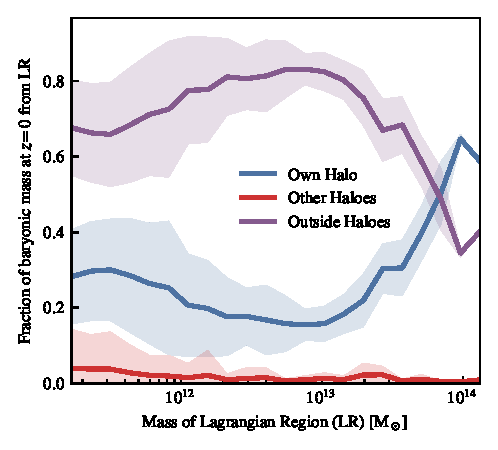
\includegraphics{figures/s50j7k/inverse_component_fraction.pdf}
	\vspace{-0.7cm}
	\caption{The fate of gas that begins in lagrangian regions, as a function of
	initial lagrangian region mass. The normalisation in this plot is incorrect
	(i.e. bins do not sum to one) because of the differing particle masses at 
	$z=0$ and the initial conditions, however the overall trends are still 
	accurate. \blue{Will include the $z=2$ line here, which
	is significantly different.} }
	\label{fig:transferoutoflrs}
\end{figure}

The clear inverse to the above discussion is to consider what happens to the gaseous
material that originated in a given lagrangian region. Now looking at the results as
a function of lagrangian region mass (this is slightly higher than the eventual
halo mass as the baryon fraction of a given halo is lower than the cosmic mean), it
is clear that there is an even more significant transfer \emph{out} of lagrangian
regions than \emph{into} halos (see Figure \ref{fig:transferoutoflrs}). Only 
approximately $20\%$ of the gas initially resident in a given lagrangian region
makes it into the $z=0$ halo. The more massive halos in the box (of which there 
are very few) manage to accrete the majority of the baryons associated with their
lagrangian region.

The relation between halo mass and transfer out of the lagranian region peaks
around $10^{12.5-13}\msolar{}$ where the efficiency of AGN feedback peaks. What
is surprising, though, is that this AGN feedback is more effective at evacuating
baryons from intermediate mass halos than stellar feedback is at evacuating
baryons from low mass halos. This is because preventative feedback also has
significant effects here, with accretion impacted by the hot IGM and CGM that
surrounds the galaxies in these halos.

\begin{figure}
	\centering
	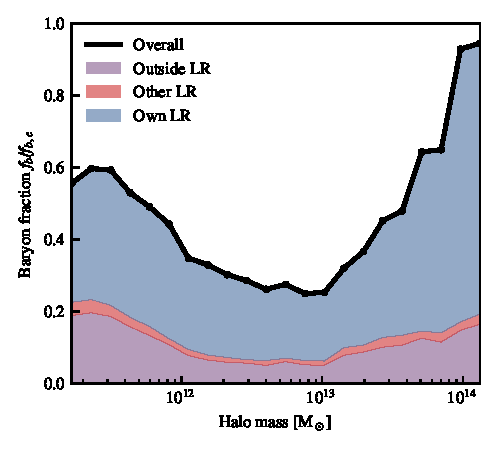
\includegraphics{figures/s50j7k/baryon_fraction_breakdown.pdf}
	\vspace{-0.7cm}
	\caption{The baryon fraction $f_b$ relative to the cosmic baryon fraction
	$f_{b, c}$ shown as a function of halo mass. The coloured bands show the
	contributions to the baryon fraction from various lagrangian components.}
	\label{fig:baryonfraction}
\end{figure}

The baryon fraction of the $z=0$ halos in Figure \ref{fig:baryonfraction}
shows, as expected, a strong dependence on halo mass ($M_H$). Halos with a
mass  $M_H > 10^{12} \msolar{}$ can have efficient AGN feedback; this has two
effects. The AGN feedback causes a the halo to become heated to $T_{\rm
vir}$, the virial temperature of the halo (typically $\sim10^{7-8}$ K for Milky
Way-mass halos). This `hot halo' acts to prevent infall from outside, a
clearly efficient pathway in \simba{} as the halo since infall from outside of
the lagrangian reigion is curtailed by 50\% in this mass region.  The other
pathway is to eject mass that was already inside the lagrangian region; this
effect is less powerful in \simba{} as gas from the lagrangian region of the
halo is only affected at the $\sim10-20\%$ level.

Once halos begin to reach $M_H > 10^{14} \msolar{}$, the potential well
becomes too deep and so the evacuation caused by AGN feedback again stops
being efficient, causing a significant increase in the retention of baryons
that originated from that halo's lagrangian region. The dependence of baryons
accreted from outside of any lagranigan region on halo mass appears to be
relatively weak, with a much less significant dip at $10^{12} \msolar{} < M_H
< 10^{14} \msolar{}$.
